\documentclass[a4paper,12pt]{article}
\usepackage[utf8]{inputenc}
\usepackage[T1]{fontenc}
\usepackage[french]{babel}
\usepackage{amsmath}
\usepackage{amsfonts}
\usepackage{amssymb} %packages inutiles pour le traitement de texte.
\usepackage{graphicx} % package à utiliser uniquement pour insérer des photos --> pas utile ici.
\usepackage{hyperref} % utile si tu veux créer des hyperliens...
\hypersetup{pdfstartview = {XYZ null null 1.00}} % pour avoir un zoom de 100% sur la liseuse PDF, c'est plus agréable !
\usepackage[hmargin=2cm,vmargin=3cm]{geometry} % hmargin et vmargin permettent de régler les marges horizontales et verticales directement.
\usepackage{wrapfig}
\usepackage{enumitem}
\usepackage{fancyhdr}
\usepackage{float}
\usepackage{eurosym}
\pagestyle{fancy}

%\setlength{\parindent}{0cm}
%\setlength{\parskip}{1ex plus 0.5ex minus 0.2ex}
\newcommand{\hsp}{\hspace{20pt}}
\newcommand{\HRule}{\rule{\linewidth}{0.5mm}}

\begin{document}
\begin{titlepage}
  \begin{sffamily}
  \begin{center}
    \begin{figure}[th]
	
\includegraphics[width=5cm]{su.png}\hfill \vspace{1cm}
	\end{figure}  	
    \vspace{1cm}
    \textsc{\LARGE DevRep : Projet Webots}\\[2cm]
    \HRule \\[0.4cm]
    { \huge \bfseries Rapport \\[0.4cm] }

    \HRule \\[2cm]
    \includegraphics[width=8cm]{webots.png} \vspace{1cm}
    \\[1cm]

    % Author and supervisor
    \begin{minipage}{0.4\textwidth}
      \begin{flushleft} \large
      %{\Large\bf\sf A.Bulteau, B.Kerléguer, M.Louart, T.Loridant, V.Perrin}
		\emph{Equipe :} \\        
        \textsc{Kimmeng Ly}\\
        \textsc{Adam Latiri}\\
      \end{flushleft}
    \end{minipage}
    \begin{minipage}{0.4\textwidth}
      \begin{flushright} \large
        \emph{Encadrants :} \\ 
        \textsc{Tewfik Ziadi}\\
        \textsc{Lom Hillah}
      \end{flushright}
    \end{minipage}

    \vfill

    % Bottom of the page
    {\large 2020 - 2021}

  \end{center}
  \end{sffamily}
\end{titlepage}
\newpage

%HEADER
\renewcommand{\headrulewidth}{1pt}
%\fancyhead[H]{\thepage}
\fancyhead[L]{
\includegraphics[scale=0.15]{su.png}}
%\fancyhead[R]{
\includegraphics[scale=0.1]{webots2.png}}
\fancyfoot[C]{Rapport - Projet Webots}
{\ \vspace{-1cm}}

\renewcommand{\contentsname}{Sommaire}
\tableofcontents
\newpage

\section{Introduction}
Dans le cadre de ce projet, nous allons étudier essentiellement la notion de \textbf{DSL}.
DSL signifie Domain Specific Language. Autrement dit, il s’agit d’un ensemble restreint de vocabulaire et de règles de grammaire qui permet de répondre à un besoin précis de description ou d’organisation de l’information.

Dans notre cas, il s'agit de développer un DSL basé sur les \textbf{diagrammes d’Arkin} mais également, par la suite, développer un générateur de code pour faciliter le
développement de petites applications robotique mobile dont \textbf{Webots}.

\subsection{Les diagrammes d'Arkin}
Les diagrammes d'Arkin sont le fruit d'une \textbf{démarche basée sur les comportements}. Un comportement est défini comme une activité primitive qui prend en entrée les données des capteurs et retourne une action à effectuer.
\\Le fait que chaque robot possède un ensemble de comportements, un système d’arbitrage est introduit afin d'intercepter les comportements et de sélectionner le comportement ayant la priorité la plus élevée.
\vspace{0.5cm}
\begin{figure}[!h]
    \center
    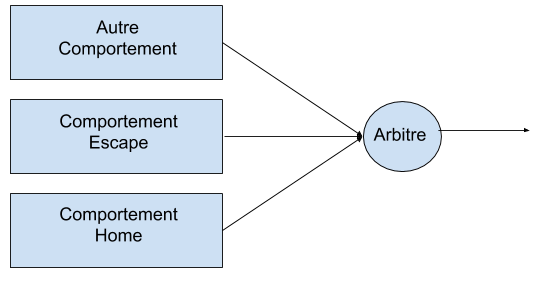
\includegraphics[width=10cm]{arkin.png}
    \caption{Diagramme Arkin}
\end{figure}
\vspace{1cm}

\subsection{Webots}
Webots est un simulateur open-source. Il permet de tester des contrôleurs pour des robots évoluant dans un monde que l’on peut modeler (dans notre projet, nous utiliserons E-puck). 
\\Le monde de Webots est en particulier capable de simuler la masse et la collision entre les objets.

\newpage
\section{Méta-modèle}
\subsection{Syntaxe abstraite}
Pour la syntaxe abstraite, nous proposons le méta-modèle suivant : 


\begin{figure}[!h]  
    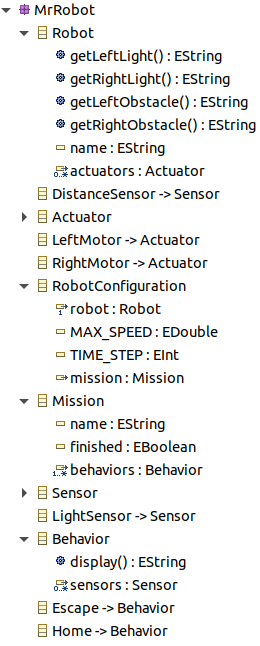
\includegraphics[width=4.5cm]{abstract_model.png}
    \caption{Méta-modèle (syntaxe abstraite)}
\end{figure}
\vspace{0.5cm}
La classe \textit{RobotConfiguration} est le point d'entrée de notre méta-modèle. Elle contient une instance de \textit{Robot}, une instance de \textit{Mission}, un attribut \textit{MAX\_{}SPEED} et un attribut \textit{TIME\_{}STEP}.
\\Un \textit{Robot} contient un ensemble d'effecteurs(\textit{Actuators}) et un ensemble de méthodes renvoyant la situation actuelle du robot, c'est-à-dire que s'il y a un obstacle ou une source de lumière sur un coté.
\\Une mission comporte un nom, \textit{SearchForLight} dans notre cas, mais aussi un ensemble de comportements. Il existe deux comportements dans notre modèle, \textit{Escape} qui consiste à éviter les obstacles et \textit{Home} qui consiste à aller vers une source de lumière, notons que le comportement \textit{Escape} est prioritaire par rapport au comportement \textit{Home}.
\\Ensuite, nous avons les capteurs. Ils sont divisés en deux catégories, les capteurs de distance et les capteurs de luminosité.
\\Et enfin, nous avons les effecteurs qui correspondent au moteur du robot. Il y a un moteur droit et un moteur gauche pour chaque robot.
\newpage

\subsection{Une syntaxe concrète}
Pour la syntaxe concrète, nous avons utilisé XText. Ci-dessous, une partie de notre syntaxe concrète :
\begin{figure}[!h]  
    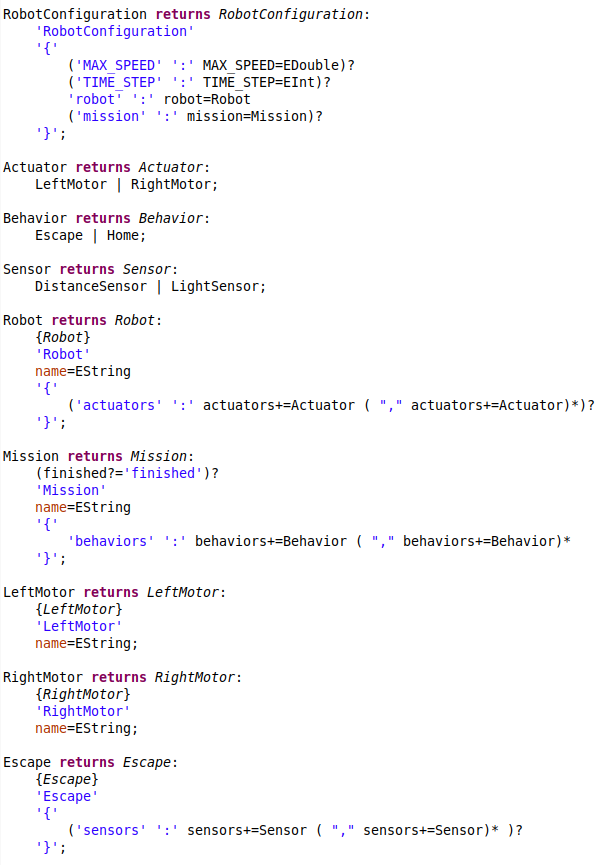
\includegraphics[width=11cm]{concrete.png}
    \caption{XText(syntaxe concrète)}
\end{figure}
\vspace{0.5cm}

Concernant la syntaxe concrète sur \textit{XText}, nous l'avons généré automatiquement à partir de notre méta-modèle \textit{ecore}. Par conséquent, nous avons les mêmes classes et chaque classe possède les mêmes attributs.
\\Une fois générée, nous pouvons apporter des modifications afin de raffiner la syntaxe et donc rendre plus visible le code.
\\Pour finir, nous devons regénérer les artefacts afin de rendre notre nouveau langage utilisable.


\newpage
\section{Implémentation d'un générateur de code}
\subsection{Java Emitter Template}
JET(Java Emitter Template) est un moteur de modèle générique qui peut être utilisé pour générer du code source SQL, XML, Java et d'autres langages à partir des modèles.
\\Nous allons donc appliquer une transformation de modèle crée vers du code java exécutable par notre robot sur Webots en utilisant
JET.
\subsection{Choix du langage et du robot}
Pour le choix du langage d’implémentation du controller pour Webots, nous avons choisi java car il nous permet d’avoir une vision objet pour la génération de code.

Pour le choix du robot, nous avons choisi le robot E-puck car celui-ci est simple et convient parfaitement à l'objectif que nous voudrions atteindre.
\subsection{Fonctionnement globale}
Pour que le robot E-puck accomplisse sa mission, il a besoin de deux types de capteurs, les capteurs de distance et les capteurs de luminosité, qui sont décrit dans notre méta-modèle.

Au début, le générateur instancie la liste des capteurs, ainsi que ses roues. Ensuite, dans une boucle while permettant de contrôler le robot à chaque intervalle de temps, on récupère les valeurs lues par les capteurs (intensité de la lumière et distance par rapport aux obstacles), et selon le comportement souhaité pour le robot, changer en conséquence la direction dans laquelle il se déplace.
\begin{figure}[!h]  
    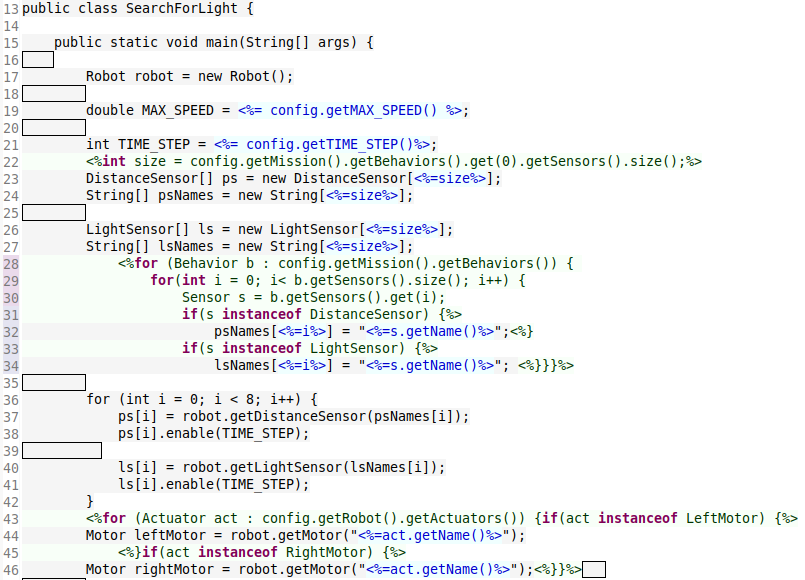
\includegraphics[width=12cm]{template.png}
    \caption{JET: une portion de notre template}
\end{figure}

\newpage
\section{Tests de validation}
\subsection{Test de la syntaxe abstraite}
Pour valider notre syntaxe abstraite, nous avons crée une instance dynamique de RobotConfiguration. A partir de cette instance nous avons ajouté un robot ainsi qu'une mission comme le montre la figure ci-dessous :

\begin{figure}[!h]  
    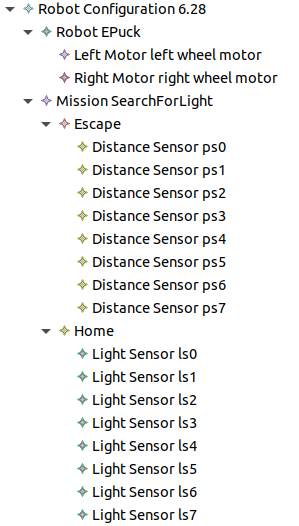
\includegraphics[width=5cm]{instance_xmi.png}
    \caption{Une instance dynamique de RobotConfiguration}
\end{figure}

%\newpage
\subsection{Test de la syntaxe concrète}
Pour valider notre syntaxe concrète, nous avons écrit, depuis une autre instance d'eclipse, un fichier \textit{.mydslx} et notre langage est bien reconnu(les mots clés définit sont colorés).
\begin{figure}[!h]  
    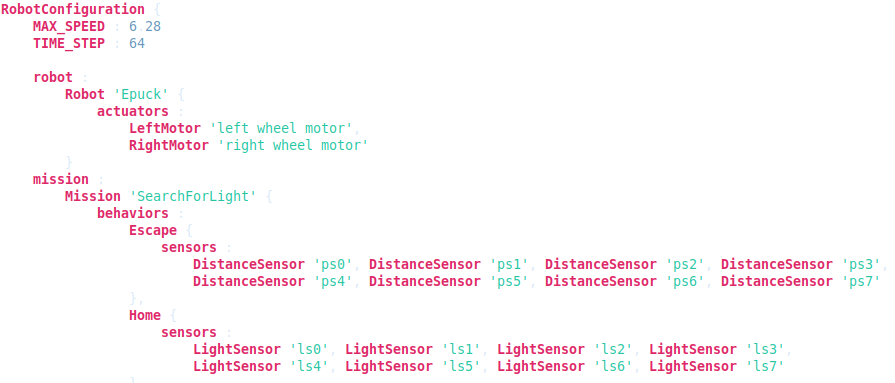
\includegraphics[width=13cm]{xtext.png}
    \caption{Utilisation de notre DSL}
\end{figure}

\subsection{Test du générateur de code}
A partir d'une méthode intermédiaire, nous avons chargé l'instance dynamique crée précédemment en une instance java et ainsi passer en paramètre à la méthode \textit{generateJavaFile} 
,qui permet de créer un fichier java, qui va utiliser notre template en utilisant l'instance fournie. 
\begin{figure}[!h]  
    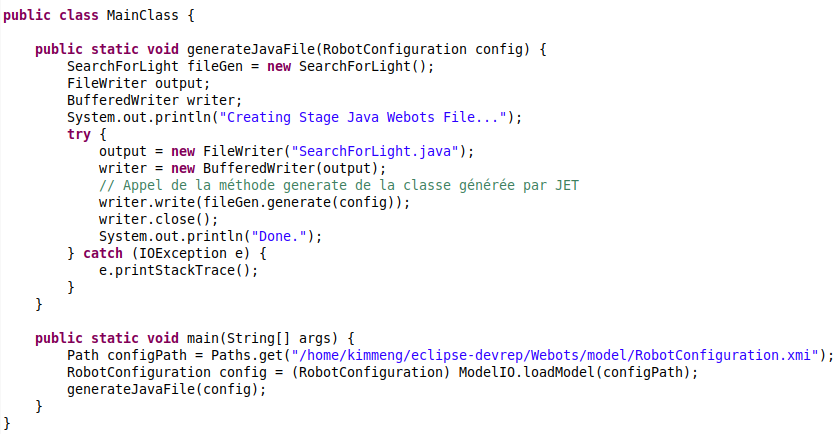
\includegraphics[width=14cm]{main.png}
    \begin{flushleft}
    La classe template va ensuite renvoyer ce code ci-dessous qui sera écrit dans un fichier java.
    \end{flushleft}
    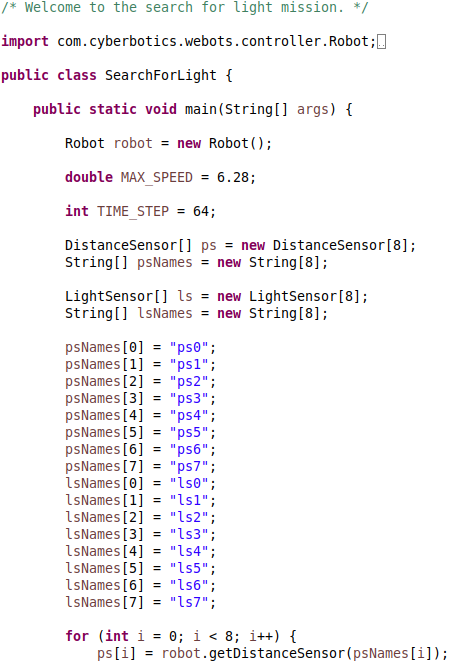
\includegraphics[width=7.5cm]{code_gen.png}
    \caption{Portion de code généré}
\end{figure}

\newpage
\subsection{Test du code produit sur Webots avec le robot E-puck}
Enfin pour valider le tout, nous avons testé le code généré sur Webots. Pour ce faire, nous avons changé le code du controlleur du robot E-puck. 
\\Et comme nous pouvons le voir, le robot poursuit bien une source de lumière tout en évitant des obstacles si ceux-ci se présentent.

\begin{figure}[!h]  
    \centering
    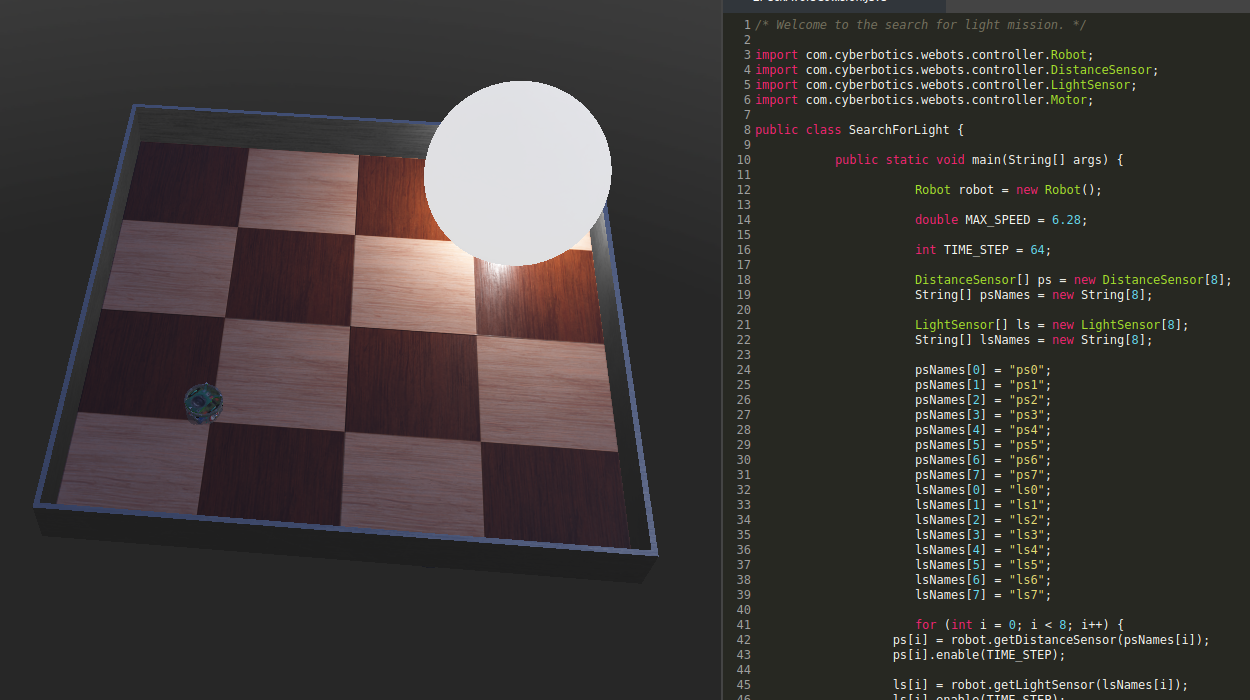
\includegraphics[width=8.4cm]{simu_1.png}
    %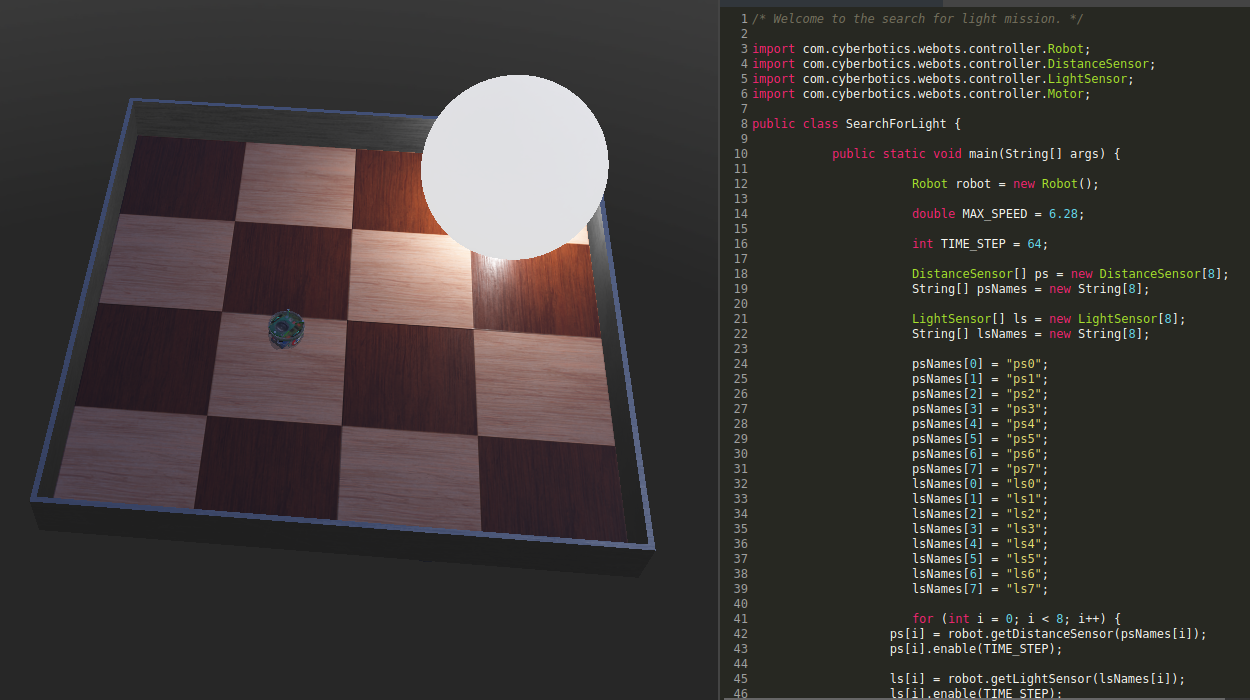
\includegraphics[width=10cm]{simu_2.png}
    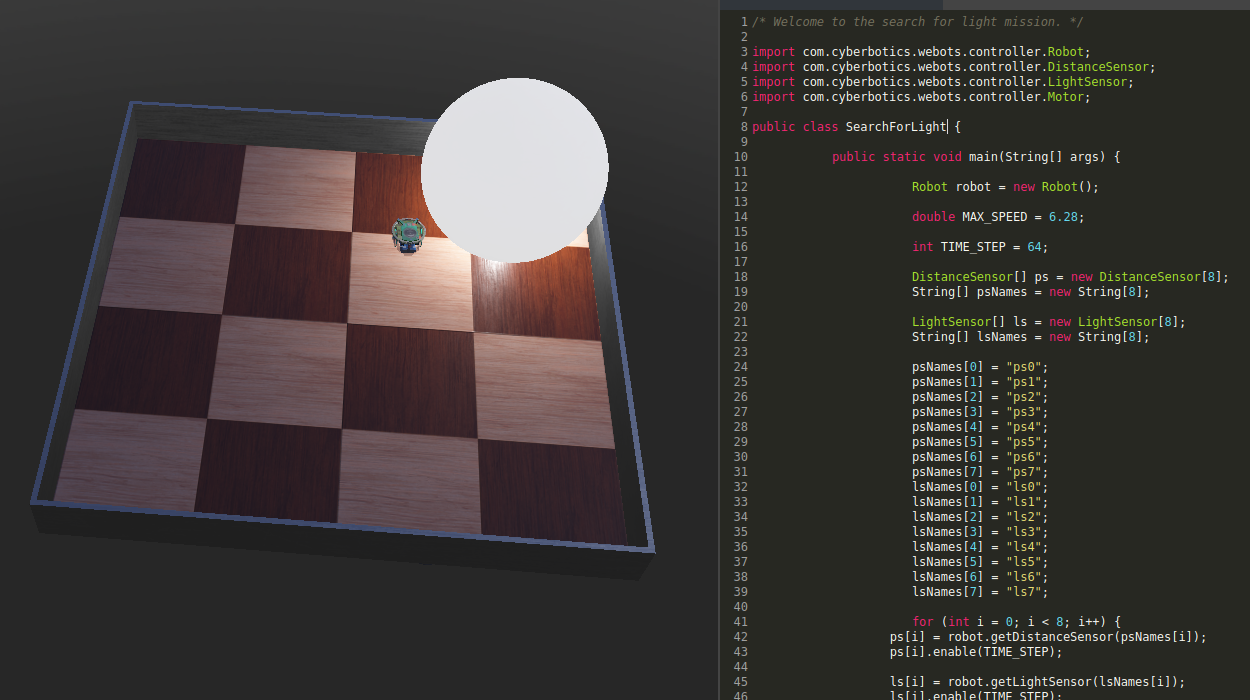
\includegraphics[width=8.4cm]{simu_3.png}
    \caption{Simulation du robot E-puck avec le code généré}
\end{figure}

\vspace{1cm}
\section{Conclusion}
En conclusion, nous avons mis au point les fonctionnalités permettant à un robot de suivre une source de lumière, d’éviter les obstacles, et d’adapter sa stratégie en fonction des valeurs lues par ses capteurs. Un utilisateur peut s’en servir avec le générateur de code pour créer un contrôleur fonctionnel, testable sur Webots.
\vspace{4cm}

\begin{thebibliography}{9}

    \bibitem{knuthwebsite} 
    Eclipse Modeling Framework (EMF),
    \\\texttt{https://www.eclipse.org/modeling/emf/}

    \bibitem{knuthwebsite} 
    Webots,
    \\\texttt{https://cyberbotics.com/}

    \bibitem{knuthwebsite} 
    JET Tutorial Part 1 (Introduction to JET),
    \\\texttt{https://www.eclipse.org/articles/Article-JET/jet\_{}tutorial1.html}

    \end{thebibliography}
    

\end{document}



